\section{Problem Analysis}\label{sec:analysis}
\subsection{Data Analysis and Preprocessing}

All problem data are geometric and rule-based; the preprocessing step converts alert
parameters into Cartesian coordinates and fixes the conventions used
throughout.\footnote{AI-assistance annotation (1/3): the coordinate-conversion and
convention-check code for this subsection was implemented with the help of an AI
pair-programming assistant; the convention decisions and the independent verification
were specified and checked by the team (see the Declaration in the Appendix and
Appendix~B).}
An alert $(\theta,R,H)$ denotes a UAV hovering at height $H$ above the ground point
\begin{equation}\label{eq:conv}
(x,y)=\bigl(50+R\cos\theta,\;50+R\sin\theta\bigr),
\end{equation}
where $\theta$ is measured counterclockwise from due east---the convention stated on
page~1 of the problem, consistent with the coordinate formula and the caption of its
Figure~2. Table~\ref{tab:targets} lists the three scheduled alerts; the disturbance alert
of Problem~4 is generated on the same rule with $H=50\,\mathrm{m}$. Field geometry
(Fig.~\ref{fig:schematic}a) comprises five prismatic buildings $B_1$--$B_5$, the dispatch
center $O=(50,50)$ and initial vehicle positions $V_1$--$V_5$. Two closed-set conventions
follow the problem statement literally: a sightline \emph{tangent} to any building edge
counts as blocked, and a disc center at exactly $1.5\,\mathrm{m}$ clearance counts as
feasible. Consequences: T2's projection sits above $B_3$'s footprint, so its LOS is
blocked when the observer hides \emph{behind} $B_3$; all targets hover above every
building, so occlusion matters only in shadow directions.

\begin{table}[!htb]\centering\small
\setlength{\tabcolsep}{3pt}
\caption{Alert targets converted by Eq.~\eqref{eq:conv} (verified independently).}
\label{tab:targets}
\begin{tabular}{cccccc}
\toprule
Target & $(\theta,R,H)$ & Ground projection $(x,y)$ & Height $H$ (m) & $r_{80}=\frac{H-2}{\tan80^\circ}$ (m) \\
\midrule
T1 & $(30^\circ,\,45,\,45)$ & $(84.6410,\,70.0000)$ & 45 & 7.5821 \\
T2 & $(150^\circ,\,45,\,35)$ & $(11.0289,\,72.5000)$ & 35 & 5.8188 \\
T3 & $(285^\circ,\,38,\,55)$ & $(59.8351,\,13.2948)$ & 55 & 9.3453 \\
T4 (Q4) & $(\theta\in[0^\circ,360^\circ),\,R\in[30,50],\,50)$ & -- & 50 & 8.4735 \\
\bottomrule
\end{tabular}
\end{table}

The radius $r_{80}$ in Table~\ref{tab:targets} is the horizontal distance at which the
elevation angle exactly hits the $80^\circ$ upper limit; it reappears in every later
question as the \emph{minimum admissible target distance}, and is the key constant that
makes both Q1's and Q2(1)'s optima analytically attainable.

\begin{figure}[!htb]\centering
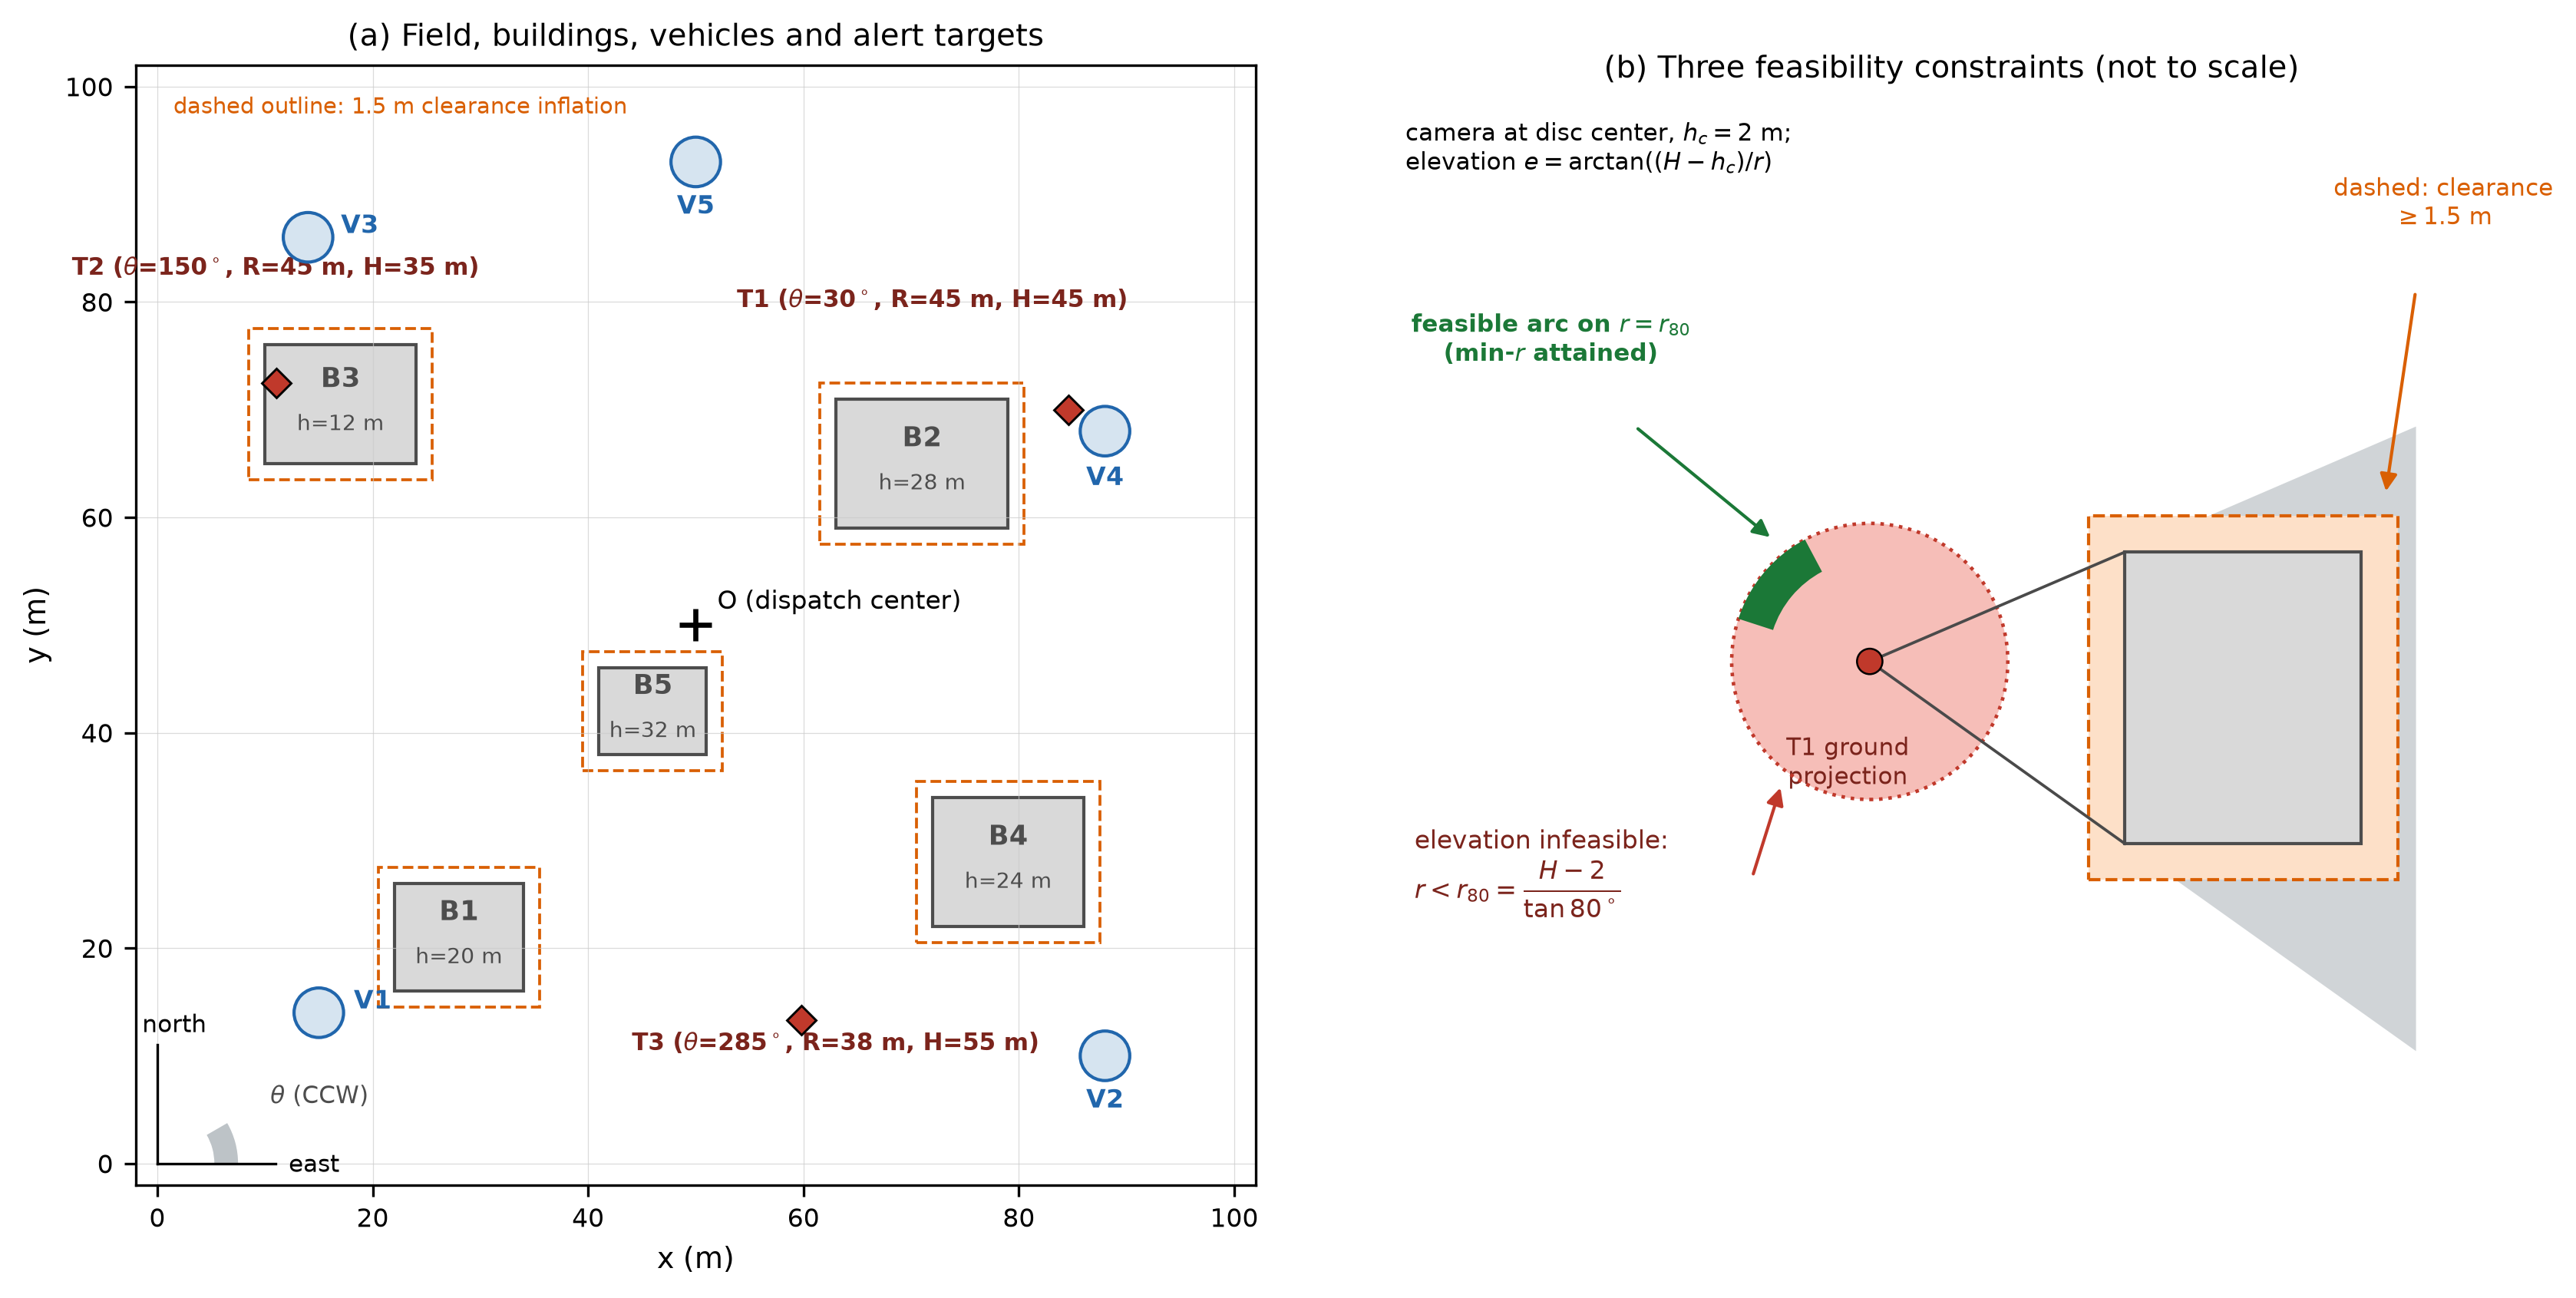
\includegraphics[width=0.62\textwidth]{fig_geometry_schematic.png}
\caption{(a) Field layout: buildings with heights, the $1.5$-m clearance inflation
(dashed), vehicles $V_1$--$V_5$ (blue) and alert targets (red diamonds).
(b) The three feasibility sieves around a target: elevation excludes $r<r_{80}$
(pink disc), an occlusion shadow (gray wedge), and the inflated footprint (orange).}
\label{fig:schematic}
\end{figure}

Figure~\ref{fig:schematic}b shows that the three constraints remove qualitatively
different disc centers---too close, hidden behind a building, or overlapping an
obstacle---so the observable region is the survivor set of three sieves. This dictates
the Q1 strategy: characterize each sieve analytically, intersect them numerically, and
audit the intersection with an independent method.

\subsection{Analysis of Question 1}

Question 1 asks for $\mathcal{F}_{T_1}$, the set of feasible camera positions for T1,
and the minimum target distance over it. Elevation alone yields the annulus
$r\ge r_{80}=7.5821\,\mathrm{m}$, so the real question is whether the $r_{80}$-circle
survives clearance and LOS anywhere---if so, the optimum is attained on a whole arc and
a tie-breaking rule becomes part of the model rather than an afterthought. We pair a
robust grid computation (for the required region map) with an analytic arc computation
on the $r_{80}$-circle (for the exact optimum), declaring the tie-break explicitly
(Section~\ref{sec:q1}).

\subsection{Analysis of Question 2(1)}

Question 2(1) is estimation theory wrapped in a discrete--continuous optimization:
choose 2 of 5 vehicles and one station per vehicle to minimize an accuracy metric under
a 30-s travel budget ($90\,\mathrm{m}$ geodesic). Bearing-only localization accuracy is
classical Fisher-information territory \cite{torrieri1984,aidala1979,kay1993}; the
problem adds feasibility---stations must lie in $\mathcal{F}_{T_2}$ and be reachable. We
adopt the root-mean-square position error $\mathrm{RMSE}=\sqrt{\operatorname{tr}C}$
(A-optimality) as primary metric---meters, comparable across pairs, directly
interpretable---with the determinant (error-ellipse area) and condition number
(anisotropy) of $C$ as diagnostics. The closed form
$\mathrm{RMSE}=\sigma_b\sqrt{d_1^2+d_2^2}/\sin\gamma$ turns the search into geometry:
the lower bound $\sigma_b\sqrt2\,r_{80}$ is attained iff both stations sit on the
$r_{80}$-circle at $\gamma=90^\circ$, reducing the continuous optimization to a
one-parameter family plus a tie-break---mirroring the structure discovered in Q1.

\subsection{Analysis of Question 2(2)}

Question 2(2) is a small-scale assign-and-sequence problem in the classical
deterministic-scheduling sense \cite{pinedo2023}: 3 alerts, 2 vehicles each, 5 vehicles,
so at least one vehicle serves two alerts; the objective is min--max on the latest
alert-start time. The combinatorial outer layer (who doubles, in which order, with which
partner) is exhaustively enumerable within the natural single-doubler family
($5\times3\times2\times4!/2=360$ structures), while the continuous inner layer (six
station coordinates) is handled by candidate screening plus best-response refinement;
both layers are evaluated by the same event-timeline simulator that Q4 reuses. We do
\emph{not} claim global optimality from enumeration alone: a valid lower bound
($3.873\,\mathrm{s}$, per-alert earliest starts ignoring resource sharing) and the
resulting gap are reported honestly. The required self-defined
\emph{nearest-assignment} baseline is defined as per-alert independent minimax station
choice with first-come--first-served assignment, so the comparison diagnoses exactly
which greedy shortcut costs how much.

\subsection{Analysis of Question 3}

Question 3 is a one-dimensional error-synthesis problem plus an inverse problem: three
independent Gaussian sources---vehicle-position error (variance growing with cumulative
travel $s$), gimbal zero bias ($0.8^\circ$) and control error ($0.6^\circ$)---enter the
pointing error $\Delta\psi$ additively to first order, so $\Delta\psi$ is Gaussian with
closed-form $\sigma_{tot}(s)$ and the reliability constraint
$P(|\Delta\psi|\le5^\circ)\ge0.95$ becomes a linear inequality in $(a,b)$ for the error
law $\sigma_{loc}(s)=a+bs$. The analytical chain is cheap to invert but rests on a
small-angle linearization; we validate it by deterministic quadrature of the exact
\texttt{atan2} angle law and exact-geometry Monte Carlo \cite{metropolis1949} (angle
wrapping, no linearization), and complement the Gaussian result with distribution-free
bounds (Chebyshev/Cantelli) to
show what normality buys. Q3 runs parallel to Q2 but feeds back a deployment insight:
the pointing-reliability limit at $r=40\,\mathrm{m}$ is compared with the separate
$90\,\mathrm{m}$ driving limit of Q2(1).

\subsection{Analysis of Question 4}

Question 4 extends the Q2(2) plan to a stochastic event stream: at $t=5\,\mathrm{s}$ a
new alert may appear (type a), one vehicle may fail (type b), and communications may be
interrupted until $t_{rec}$ (type c), singly or combined. The evaluation metric is
lexicographic---completion ratio $\eta=k/N$ first, then the latest start $t_{last}$
(capped at $60\,\mathrm{s}$ when any open alert can never start)---and the comparison is
against \emph{retaining} the original commands ($P_0$). A compact scenario family
(86 scenarios) covers the full parameter domain of (a) on a $12\times3$ grid, all five
failures of (b), multiple recovery times of (c), and worst-case combinations located by
a hard-sector probe; three strategies are evaluated---$P_0$ (retain), $P_1$
(event-triggered full re-optimization sharing Q2(2)'s machinery) and $P_2$
(an interpretable rule-based greedy)---in the spirit of dynamic multi-robot task
allocation under uncertainty \cite{choudhury2022,chakraa2023}. Pairing a proactive
optimizer with a rule-based fallback lets us attribute \emph{when} and \emph{why}
rescheduling pays---a value-boundary analysis rather than a single average number.

\begin{figure}[!htb]\centering
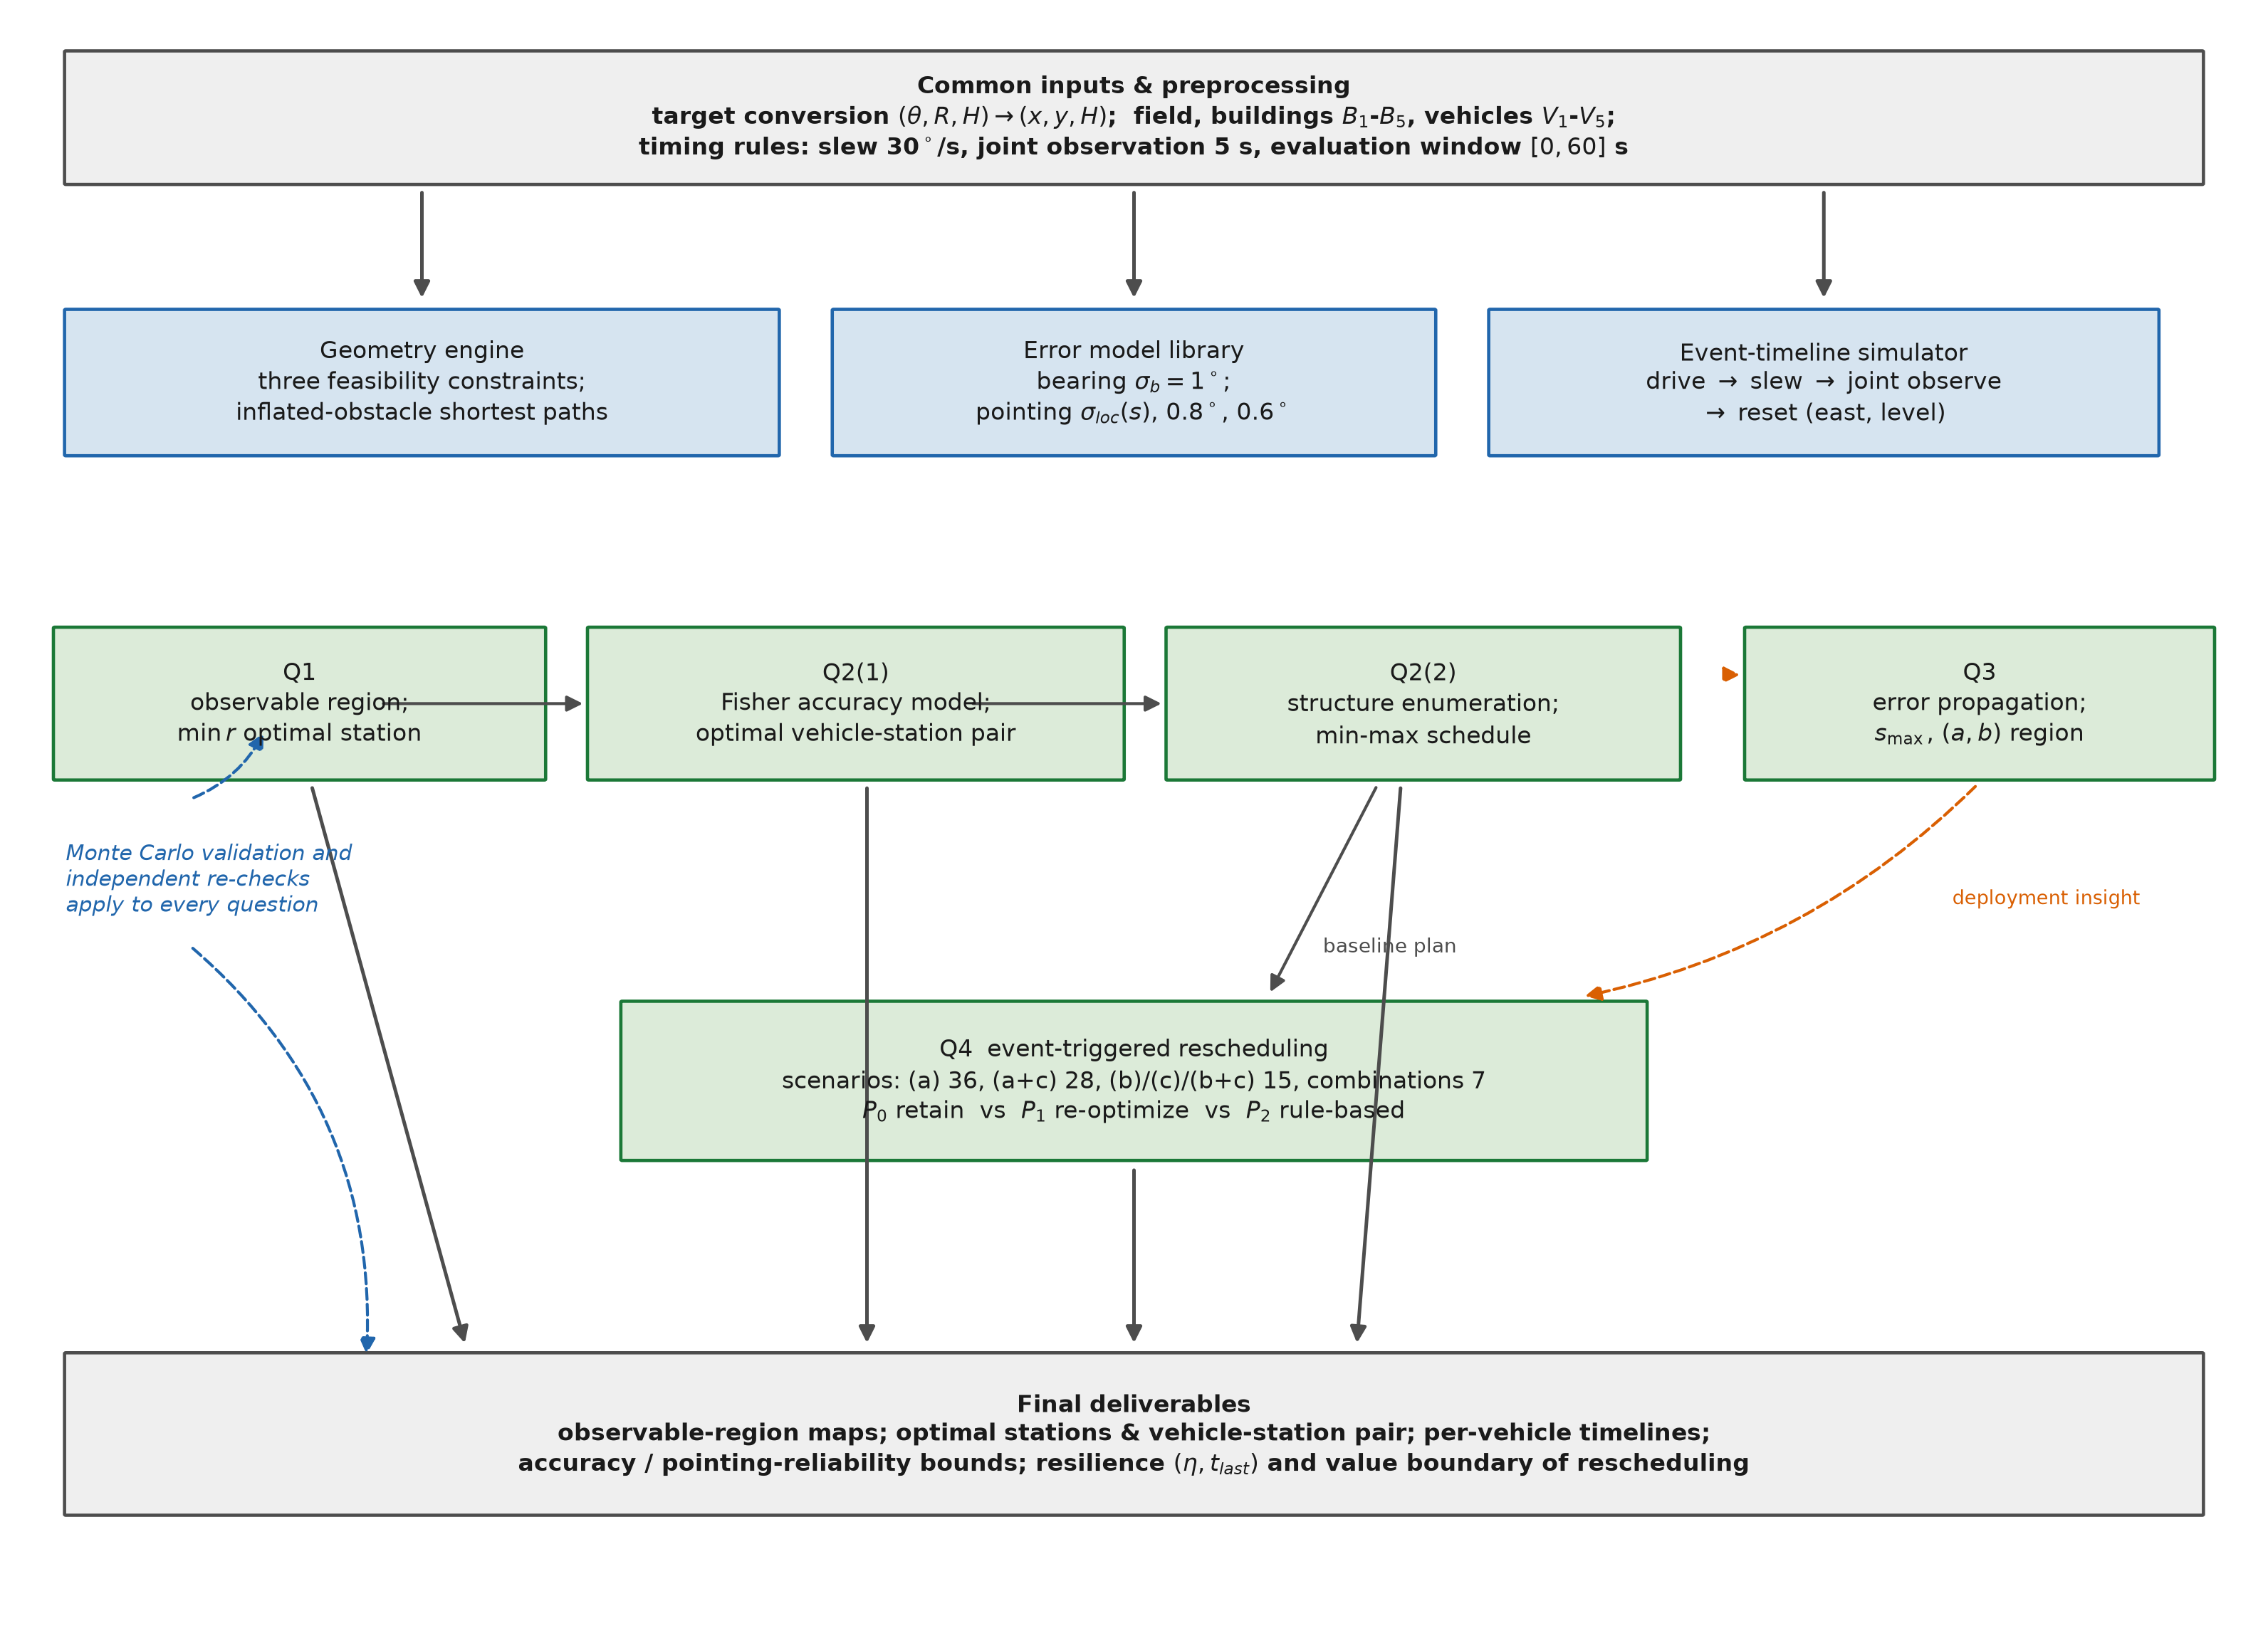
\includegraphics[width=0.56\textwidth]{fig_framework.png}
\caption{Overall technical route. Three shared engines (blue) serve all questions
(green); dashed arrows are cross-question transfers: Q3's deployment insight feeds the
schedule discussion, Q2(2)'s plan is Q4's baseline, and every question carries its own
Monte Carlo / independent re-check loop.}
\label{fig:framework}
\end{figure}

Figure~\ref{fig:framework} shows the whole pipeline. The two arrows into Q4---one solid
(baseline plan) and one dashed (deployment insight)---embody the framework's central
claim: scheduling decisions and error mechanics are two views of the same geometry, and
one shared simulator is what makes the Q4 comparison meaningful.

\subsection{Method-Selection Summary}

Table~\ref{tab:methodsel} consolidates, for each question, the candidate approaches
weighed against the selected one; the decisive criterion is always the metric the
problem statement itself asks for (feasible-region fidelity, localization accuracy,
latest alert start, pointing reliability, and the lexicographic $(\eta,t_{last})$
pair), and each selection is backed by evidence already reported in the corresponding
section---no untested alternative is claimed superior or inferior beyond what the
tables in Sections~\ref{sec:q1}--\ref{sec:q4} show.

\begin{table}[!htb]\centering\footnotesize
\setlength{\tabcolsep}{3.5pt}
\caption{Candidate approaches considered per question and the selection criterion.}
\label{tab:methodsel}
\begin{tabular}{p{0.065\textwidth}p{0.36\textwidth}p{0.22\textwidth}p{0.27\textwidth}}
\toprule
Q & Candidates weighed & Selected & Decisive reason \\
\midrule
Q1 & full grid enumeration; analytic $r_{80}$-circle arc audit; random feasible-set
sampling & grid map $+$ analytic arc audit & the map is required; the arc audit
\emph{certifies} that the bound $r_{80}$ is attained, which sampling cannot \\
Q2(1) & Fisher/CRLB metric; least-squares trilateration; weighted intersection
estimator & Fisher $\mathrm{RMSE}=\sqrt{\operatorname{tr}C}$ & closed form, attainable
lower bound, $\propto\sigma_b$ so the pair choice is noise-level free \\
Q2(2) & min--max makespan; total-completion-time; list scheduling & min--max epigraph
(Eq.~\eqref{eq:minmax}) & matches the required objective verbatim; total-time variants
optimize a different (unasked) quantity \\
Q3 & analytic linear chain; exact quadrature $+$ Monte Carlo; distribution-free bounds
& analytic chain $+$ full-geometry validation $+$ Chebyshev/Cantelli contrast & the chain
is directly invertible to the $(a,b)$ region; quadrature and MC quantify its approximation
error; the free bounds price the normality assumption \\
Q4 & $P_1$ enumeration $+$ coordinate descent; rule-based greedy ($P_2$); re-enumerate
everything at every event & event-triggered $P_1$ with $P_2$ fallback vs.\ $P_0$ &
lexicographic $(\eta,t_{last})$; the pairing attributes \emph{when} rescheduling pays
(the value boundary) \\
\bottomrule
\end{tabular}
\end{table}
